\documentclass[12pt,a4paper]{article}

\usepackage[utf8]{inputenc}
\usepackage[T1,T2A]{fontenc}
\usepackage[english,russian]{babel}
\usepackage[margin=2cm]{geometry}
\usepackage{graphicx}
\usepackage{caption}
\usepackage{subcaption}
\usepackage{float}
\usepackage{hyperref}
\usepackage{setspace}

\hypersetup{
    colorlinks=true,
    linkcolor=black,
    urlcolor=blue,
    citecolor=black
}

\captionsetup{font=small,labelfont=bf,skip=4pt}
\setlength{\parindent}{1.25em}
\linespread{1.1}\selectfont
\setlength{\intextsep}{6pt}
\setlength{\textfloatsep}{6pt}

\begin{document}

\selectlanguage{english}

% ------------------------------------------------------------
% Title page
% ------------------------------------------------------------
\begin{titlepage}
    \centering
    \vspace*{2.5cm}

    \rule{\linewidth}{1.5pt}\\[0.4cm]
    {\LARGE\bfseries Design of a Comprehensive Web-Based\\[0.2cm]
    Academic Management Platform\\[0.2cm]
    with Integrated Intelligent Features\\[0.2cm]
    as an Alternative for Traditional LMS\par}
    \rule{\linewidth}{1.5pt}\\[1.2cm]

    {\Large\scshape Diploma Thesis\par}

    \vspace{1cm}
    {\large By\par}
    \vspace{0.3cm}
    {\scshape\Large Olzhas Karabekov\\[0.15cm]
    Askat Narinbetov\\[0.15cm]
    Nurislam Baltabekov\par}

    \vspace{1cm}
    
\includegraphics[width=0.25\linewidth]{figures/aitu-logo.jpg}

    \vspace{0.6cm}
    {\large\bfseries School of Software Engineering\\
    \scshape Astana IT University\par}

    \vfill
    {6B0613 --- Software Engineering\\
    Supervisor: Zhaksylyk Kozhakhmet\par}

    \vspace{0.6cm}
    {\scshape\large June 2026\\
    Astana\par}
\end{titlepage}

% ------------------------------------------------------------
% Technical Overview
% ------------------------------------------------------------
\begin{center}
    {\Large\bfseries Technical Overview}
\end{center}
\vspace{0.2cm}

\textbf{Context and motivation.} The diploma project resulted in the
development of \textbf{UniLMS} --- a comprehensive web-based academic platform
built as a modern alternative to traditional learning management systems such
as Moodle, Canvas, and Blackboard. An empirical survey of 326 stakeholders in
Kazakhstan (209 students and 117 teachers) confirmed three pain points:
72.7\,\% of respondents miss deadlines in their current systems, 59.2\,\% want
a single unified platform, and 69.9\,\% are willing to adopt a
university-specific LMS. These findings, together with a competitive analysis
of seven existing platforms, defined three guiding principles: a contemporary
user experience, native artificial-intelligence integration in core academic
workflows, and complete trilingual coverage in English, Russian, and Kazakh.

\textbf{Architecture.} The system is delivered as a modular monolith with
three clearly separated layers and ships as a three-service Docker Compose
stack. The presentation layer is built with \textbf{Next.js 14} (App Router),
\textbf{Tailwind CSS 3.4}, \textbf{TanStack Query 5} for server-state
management, and \textbf{Framer Motion} for transitions. A custom design system
based on the OKLCH color space provides perceptually uniform gradients, dual
themes (forest light, violet dark), a density toggle, and a typography scale
built on Geist and Instrument Serif. The application layer is implemented in
\textbf{NestJS 10} with modular architecture, dependency injection, DTO
validation through class-validator and Zod, role-based access control for
student, teacher, and administrator roles, and Server-Sent Events for
sub-second real-time notifications. \textbf{PostgreSQL 15} with \textbf{Prisma
5.22} forms the data layer, with fourteen domain models, ACID transactions,
full-text search, and automatic migrations on container startup.

\textbf{AI module.} The intelligent layer is powered by \textbf{Anthropic
Claude} and exposes five production endpoints: structured assignment feedback
with strengths and improvement areas; topic-based quiz generation; course
summarization with workload estimation; individual student performance
analysis with low / medium / high risk scoring; and a streaming AI chat
assistant that delivers responses token by token through SSE and supports
client-side cancellation via \texttt{AbortController}. Every endpoint accepts
a language parameter, and a built-in demo mode allows the platform to run
without any external API key.

\textbf{Security, localization, and deployment.} Authentication relies on JWT
access and refresh tokens stored in httpOnly cookies, with bcrypt hashing,
refresh-token rotation, Helmet headers, and a Throttler rate limit of one
hundred requests per minute. Every administrative action is recorded in an
immutable audit log. Localization covers UI strings, AI prompts and replies,
e-mails, and date / number formatting through the \textbf{Intl} API with the
\texttt{kk-KZ} locale. End-to-end tests use Jest and Supertest, the project
compiles in strict TypeScript mode with zero errors, and the entire stack
launches with a single \texttt{docker compose up} command.

% ------------------------------------------------------------
% Figures — Page 3: Authentication and dashboards
% ------------------------------------------------------------
\newpage

\begin{figure}[H]
    \centering
    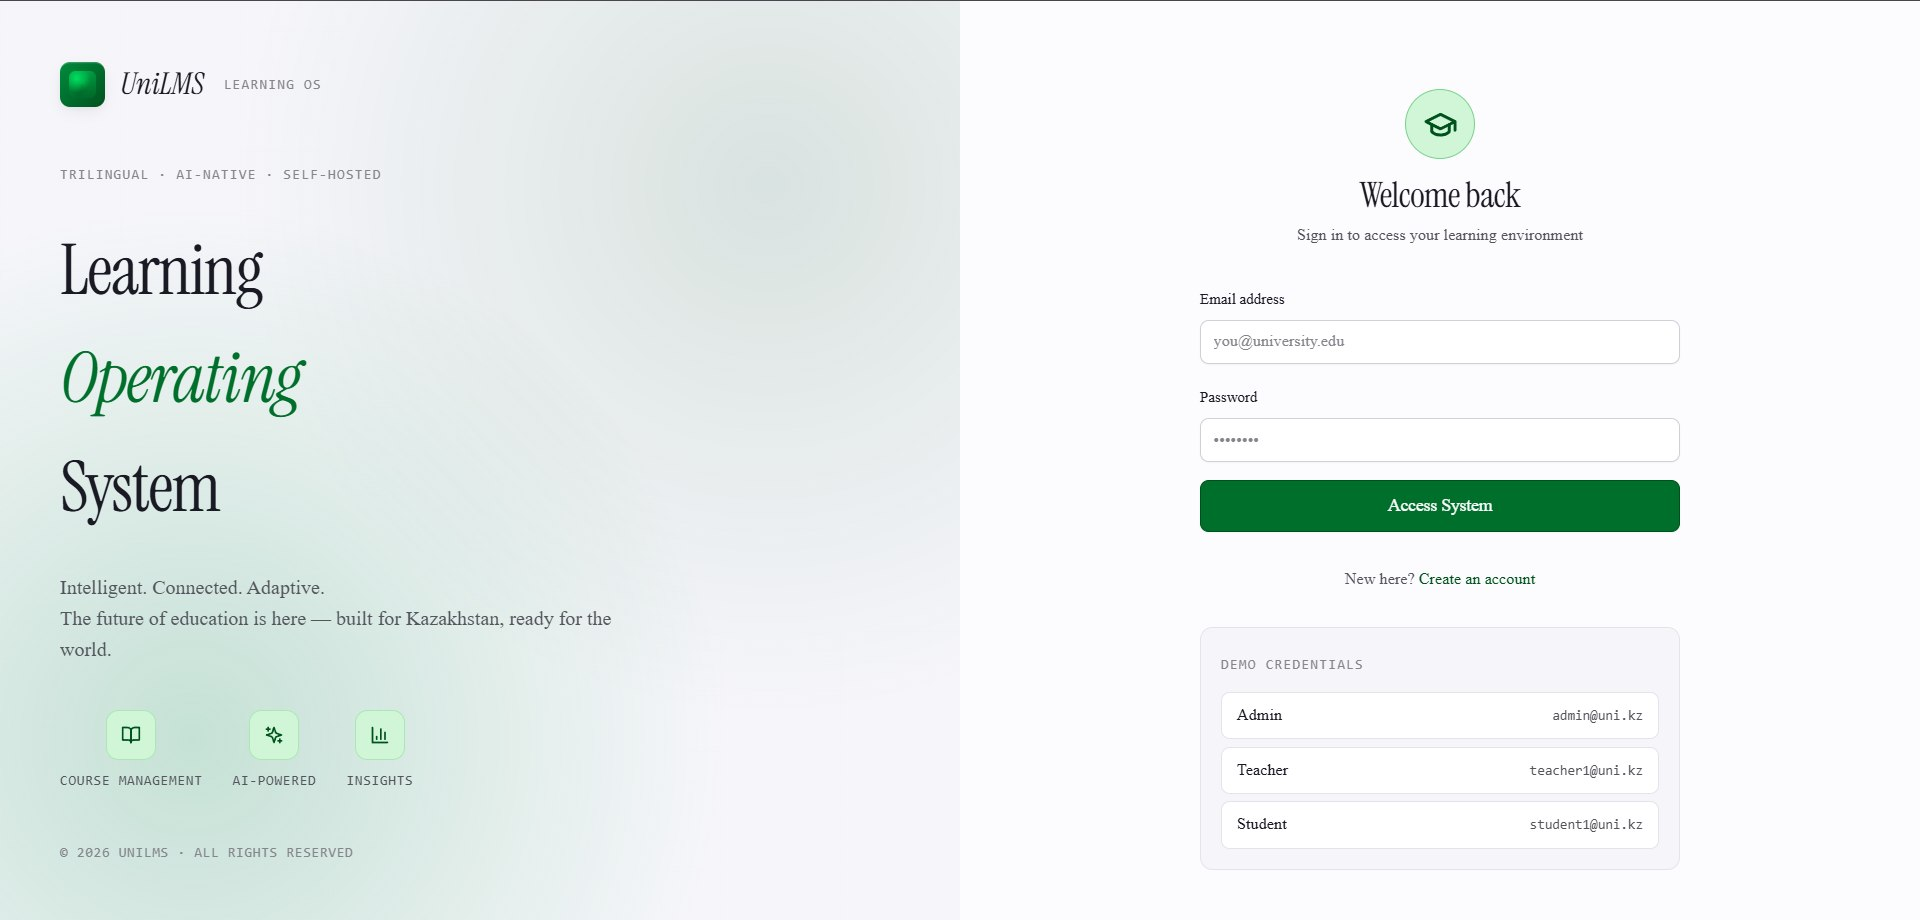
\includegraphics[width=0.65\linewidth,height=4.4cm,keepaspectratio]{figures/02-auth-login.jpg}
    \caption{Authentication screen with email/password login}
\end{figure}

The login screen is the entry point of the platform and demonstrates the
custom design system in action: an Instrument Serif heading, a clean form
built from primitives of the design system, and an inline error-handling
pattern shared across the application. Authentication itself is performed
against the NestJS backend using a JWT pair stored in httpOnly cookies, with
bcrypt password verification and refresh-token rotation on every renewal.

\begin{figure}[H]
    \centering
    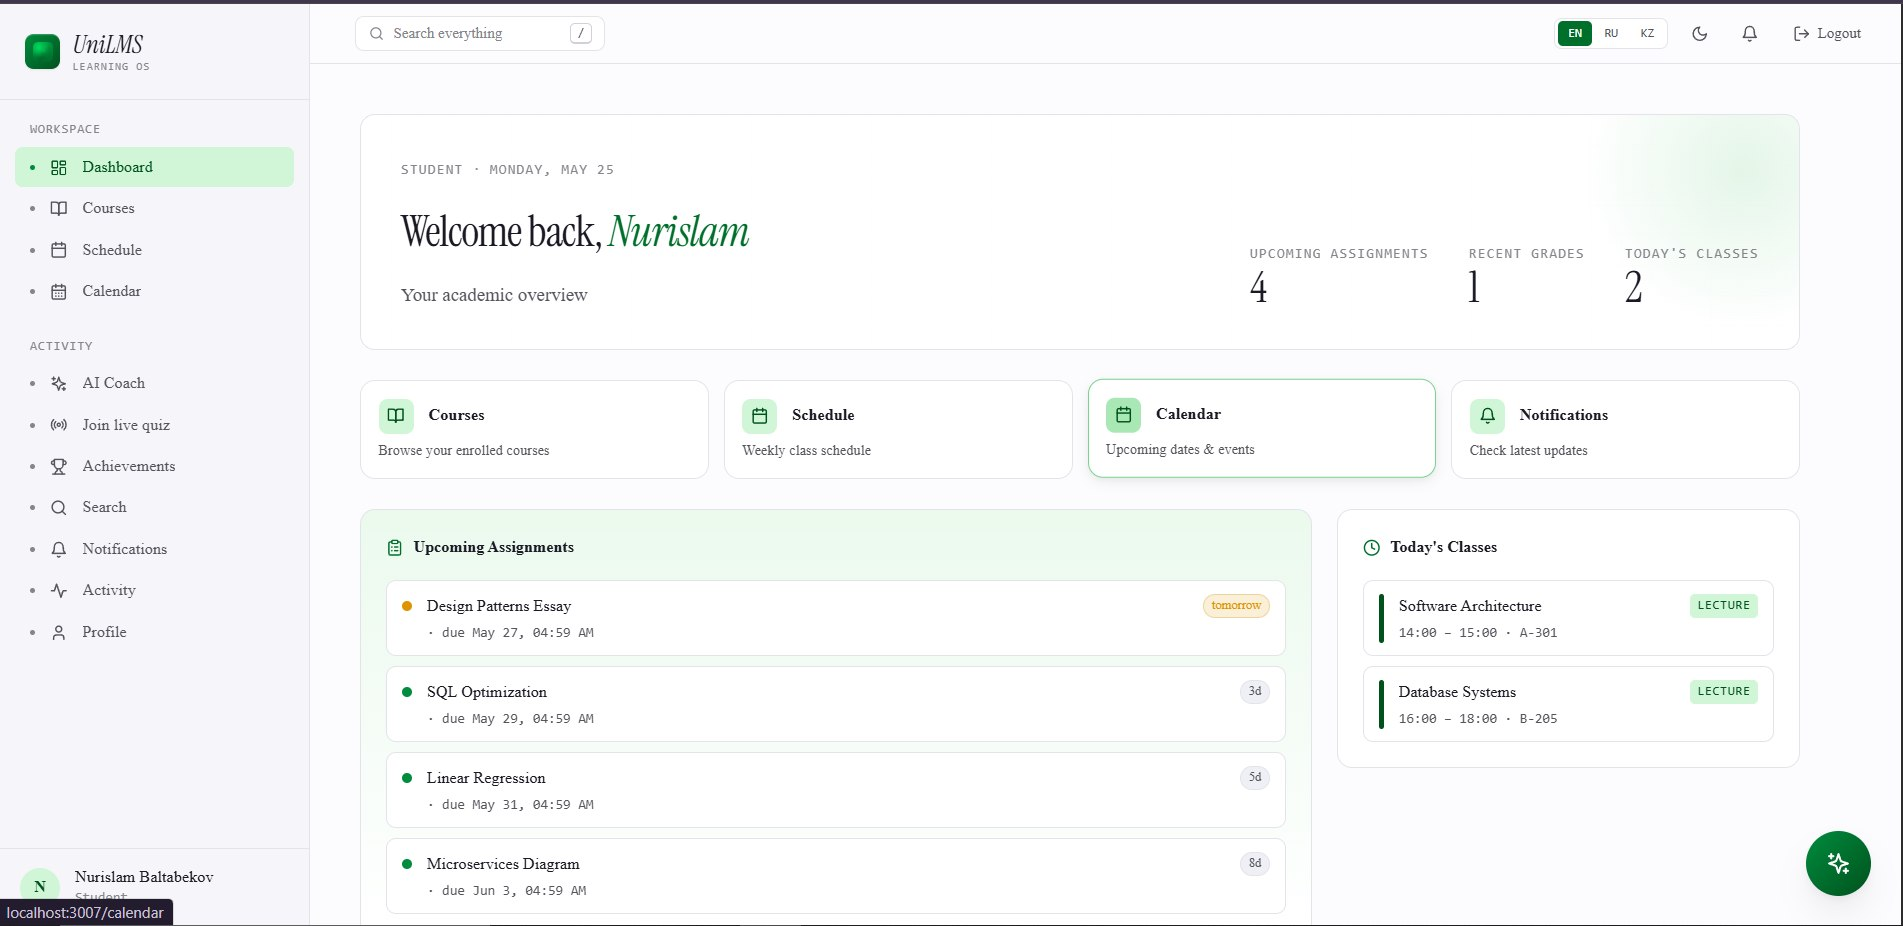
\includegraphics[width=0.85\linewidth,height=4.4cm,keepaspectratio]{figures/04-dashboard-student.jpg}
    \caption{Student dashboard with active courses, deadlines, and recent activity}
\end{figure}

The student dashboard aggregates the most important information for a learner
in a single view: enrolled courses with progress indicators, upcoming
assignment deadlines, recent grades, and unread notifications. Every widget
is rendered with optimistic UI through TanStack Query so that interactions
remain instantaneous even on a slow connection.

\begin{figure}[H]
    \centering
    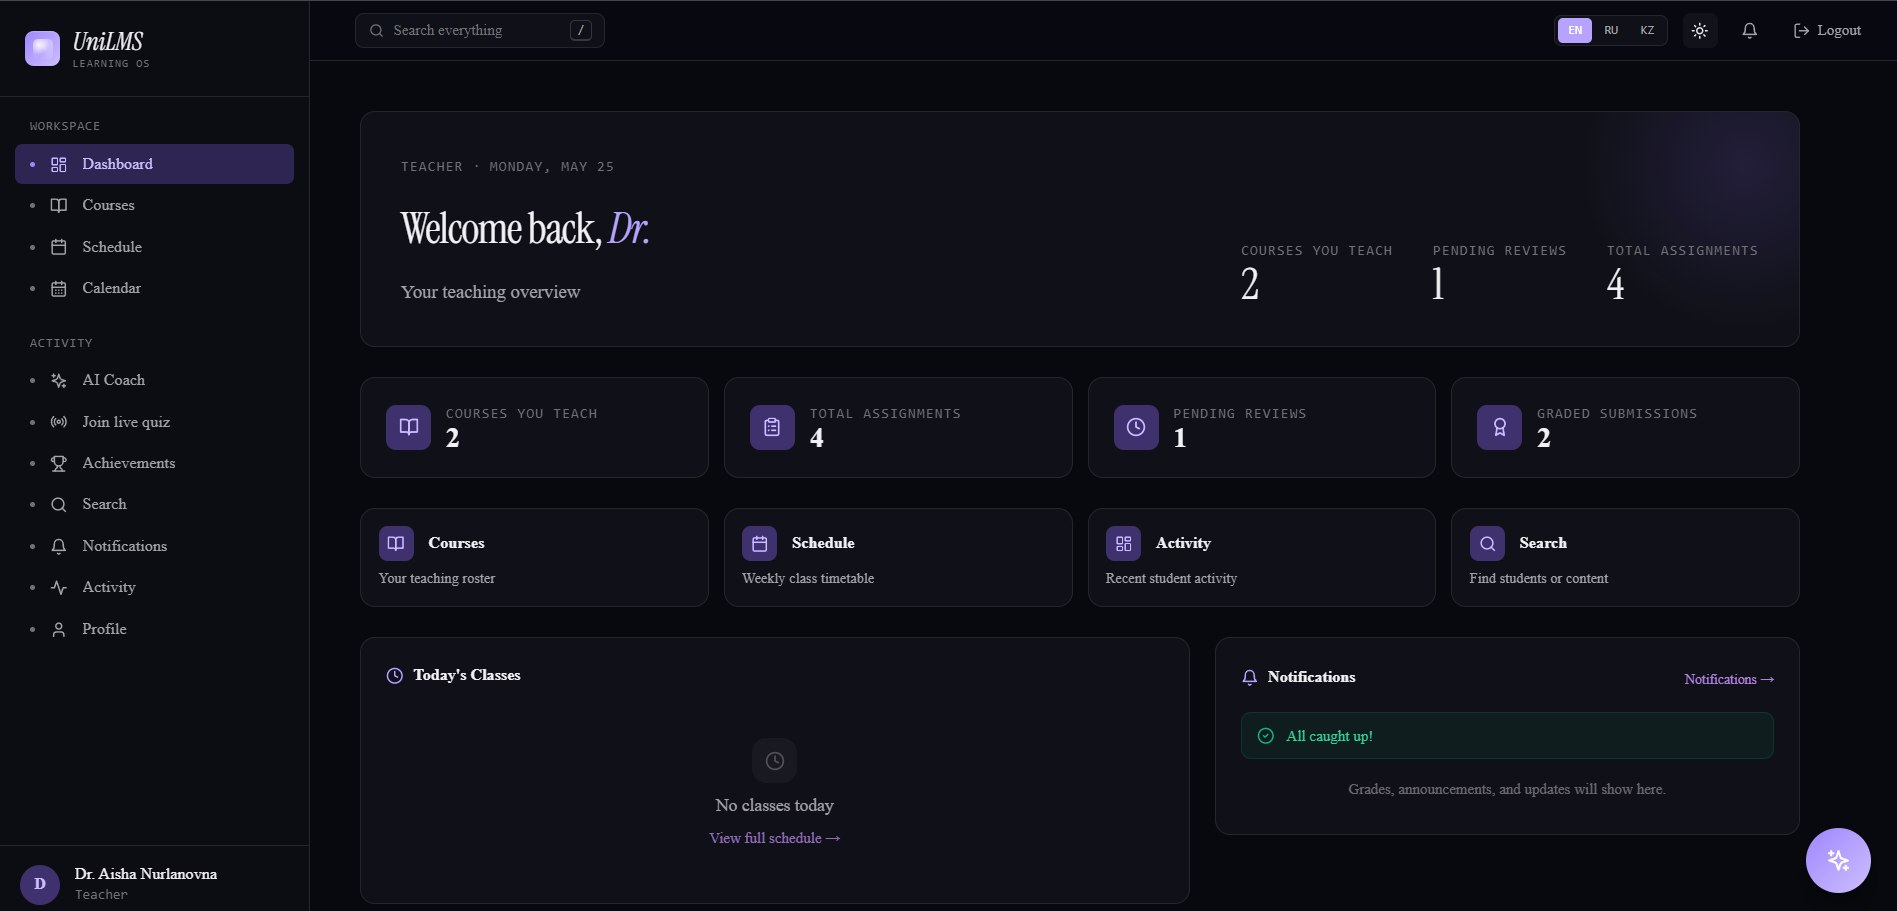
\includegraphics[width=0.85\linewidth,height=4.4cm,keepaspectratio]{figures/05-dashboard-teacher.jpg}
    \caption{Teacher dashboard with course overview and pending submissions}
\end{figure}

The teacher dashboard mirrors the student view but is oriented toward
instruction: it surfaces the number of pending submissions to grade, average
class performance per course, and quick actions for creating new assignments
or quizzes. Role-based access control enforced on the NestJS side guarantees
that only users with the teacher role can reach this route.

% ------------------------------------------------------------
% Figures — Page 4: Courses, assignments, and the first AI feature
% ------------------------------------------------------------
\newpage

\begin{figure}[H]
    \centering
    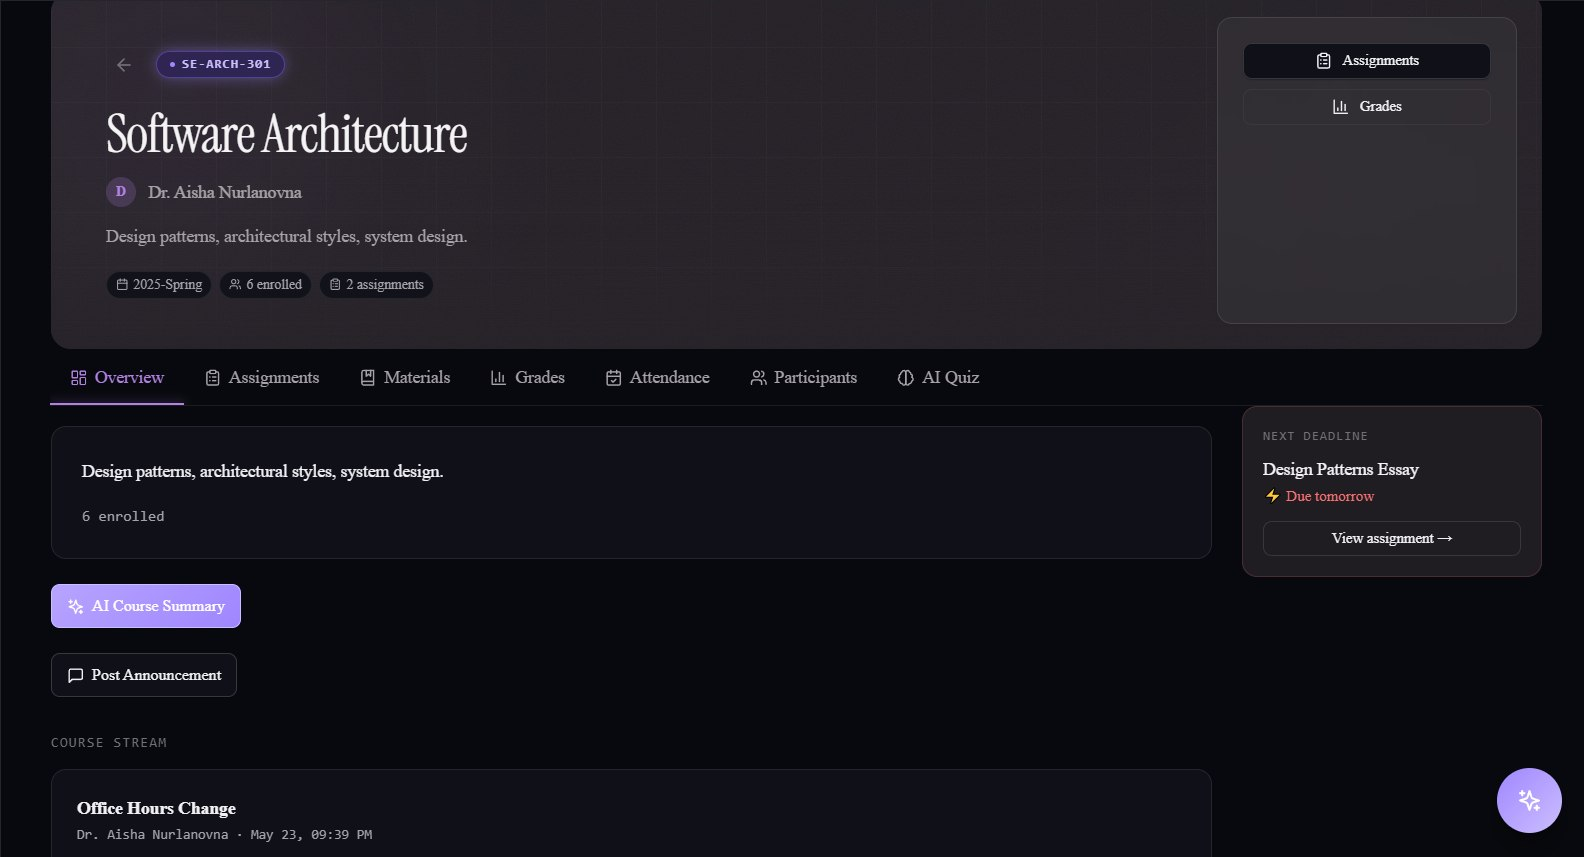
\includegraphics[width=0.85\linewidth,height=4.4cm,keepaspectratio]{figures/07-course-detail.jpg}
    \caption{Course detail page with materials, modules, and progress tracking}
\end{figure}

The course detail page is the central learning hub. It presents a syllabus
broken down into modules, downloadable materials, embedded videos, and a
progress tracker that updates as the student completes activities. The same
page acts as the teacher's content-management interface: editable in place
under the teacher role, read-only under the student role.

\begin{figure}[H]
    \centering
    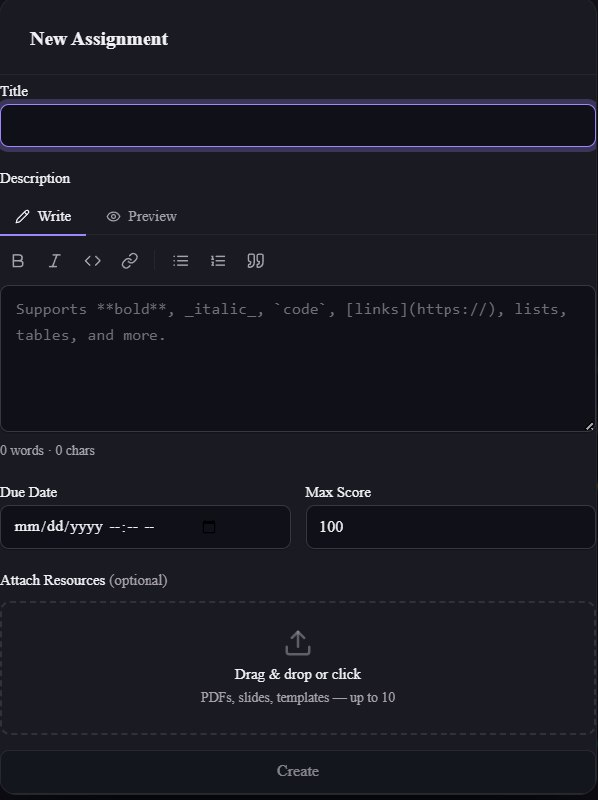
\includegraphics[width=0.85\linewidth,height=4.4cm,keepaspectratio]{figures/09-assignment-create.jpg}
    \caption{Assignment creation interface from the teacher perspective}
\end{figure}

When a teacher creates a new assignment, the form collects the title,
description, attachments, allowed file types, due date, and grading scheme.
All values are validated on both the client (Zod schema) and the server
(class-validator DTO) so that invalid data can never reach the database.
Created assignments immediately trigger SSE notifications to enrolled
students.

\begin{figure}[H]
    \centering
    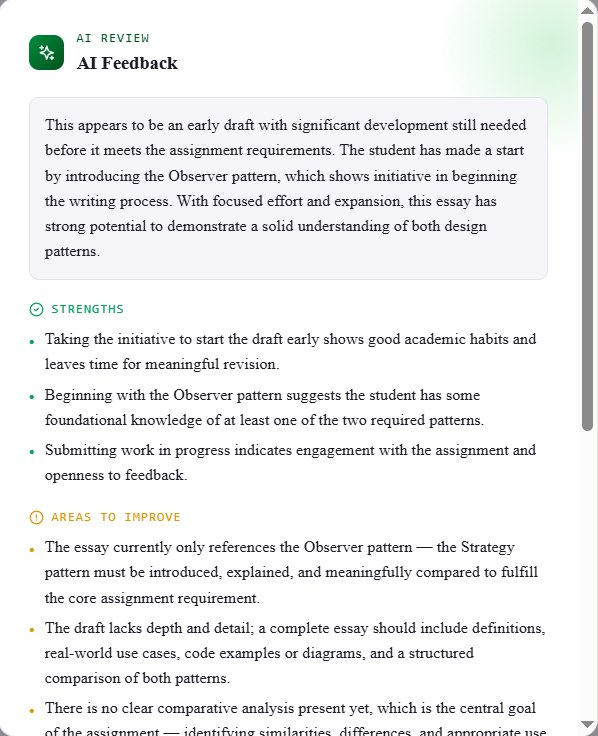
\includegraphics[width=0.85\linewidth,height=4.4cm,keepaspectratio]{figures/10-ai-feedback.jpg}
    \caption{AI-generated structured feedback on a student submission}
\end{figure}

The first of five AI endpoints generates structured feedback for a student
submission. The model returns an overall assessment, a list of strengths,
a list of areas that require improvement, and concrete actionable
suggestions. The output is validated at runtime through a Zod schema, which
guarantees that downstream UI code always receives well-formed data.

% ------------------------------------------------------------
% Figures — Page 5: Remaining four AI endpoints
% ------------------------------------------------------------
\newpage

\begin{figure}[H]
    \centering
    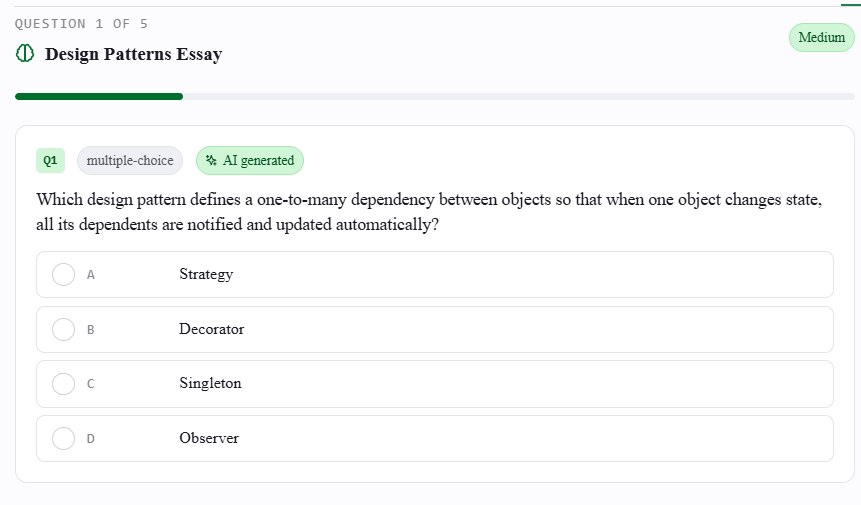
\includegraphics[width=0.85\linewidth,height=4.4cm,keepaspectratio]{figures/11-ai-quiz-gen.jpg}
    \caption{AI quiz generation with topic, count, difficulty, and language}
\end{figure}

The quiz generator accepts a topic, the desired number of questions, a
difficulty level, and a target language (EN, RU, or KZ). Anthropic Claude
synthesizes a quiz with multiple-choice questions, correct answers, and
short explanations. The result can be assigned to a course with one click,
which turns the AI-generated content into a regular interactive activity.

\begin{figure}[H]
    \centering
    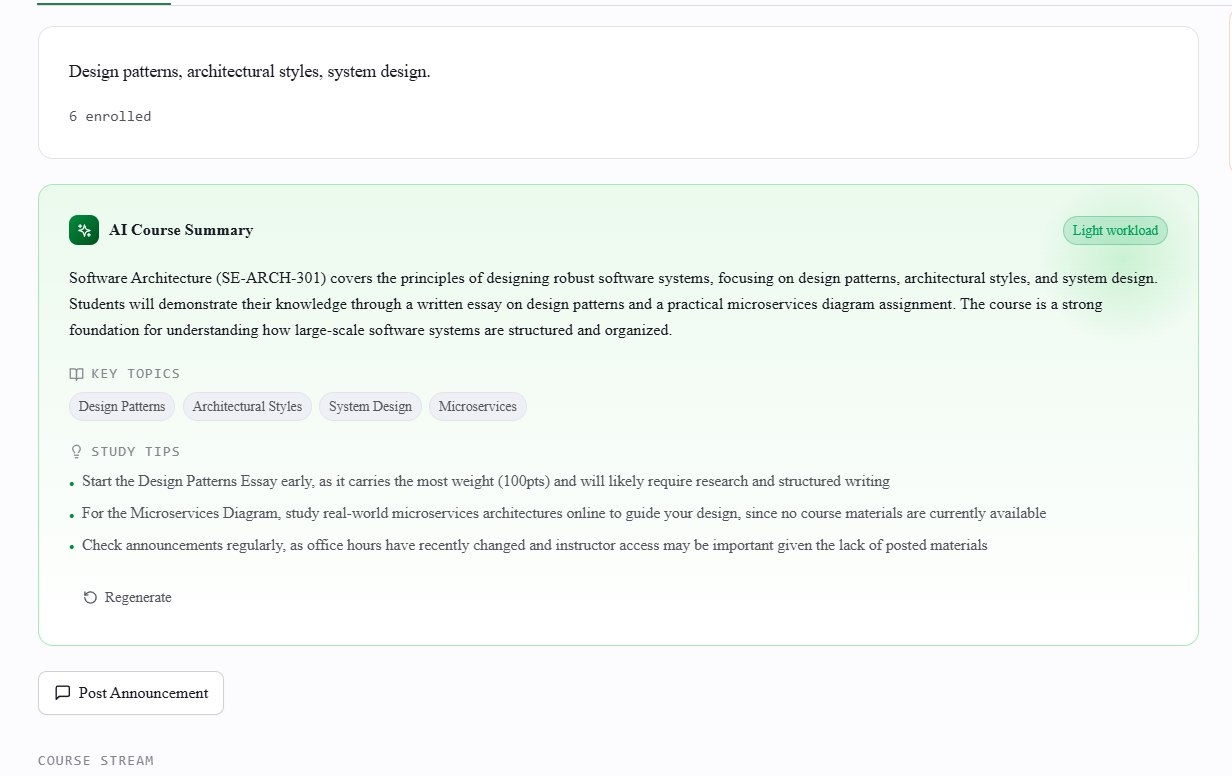
\includegraphics[width=0.85\linewidth,height=4.4cm,keepaspectratio]{figures/12-ai-course-summary.jpg}
    \caption{AI-generated course summary with key topics and workload estimation}
\end{figure}

Course summarization compresses an entire course into a synthesized overview
containing key topics, study tips, and a workload estimation classified as
light, moderate, or heavy. Teachers use this view to refine their curriculum;
students use it for last-minute revision or to decide whether to enrol.

\begin{figure}[H]
    \centering
    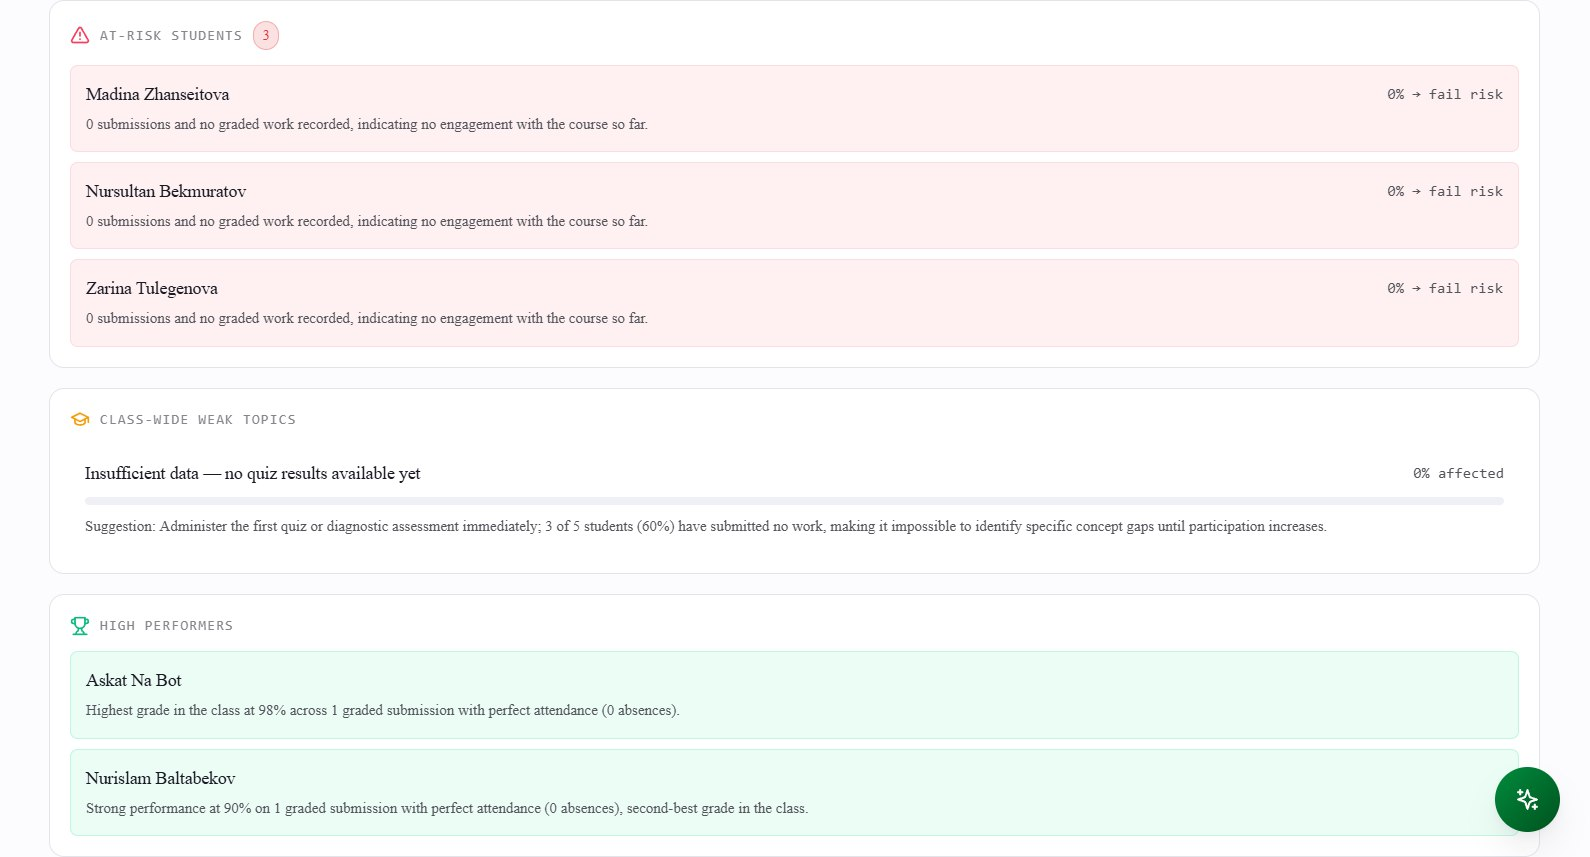
\includegraphics[width=0.85\linewidth,height=4.4cm,keepaspectratio]{figures/13-ai-student-analysis.jpg}
    \caption{AI Student Analysis screen with risk level and recommendations}
\end{figure}

Student Analysis combines grades, submission timeliness, and participation
metrics, then asks the model to classify the learner's risk level as low,
medium, or high and to produce a list of personalized recommendations. This
feature allows teachers to intervene early with students who would otherwise
silently drift off track.

% ------------------------------------------------------------
% Figures — Page 6: Chat, schedule, admin
% ------------------------------------------------------------
\newpage

\begin{figure}[H]
    \centering
    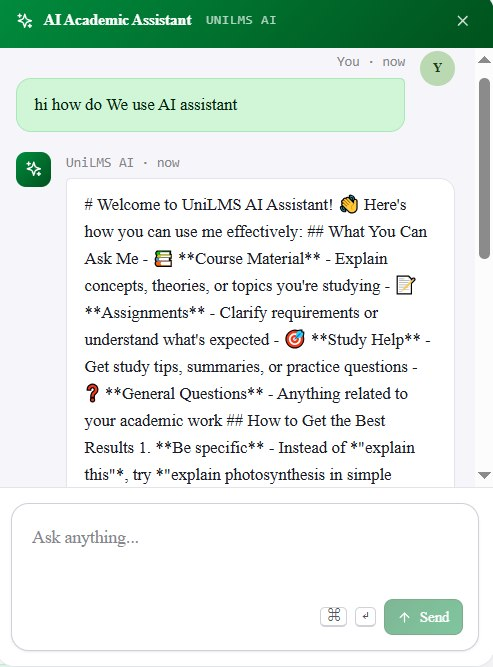
\includegraphics[width=0.85\linewidth,height=4.4cm,keepaspectratio]{figures/14-ai-chat.jpg}
    \caption{Streaming AI chat assistant with Server-Sent Events}
\end{figure}

The streaming AI chat is the most interactive feature: it delivers responses
token by token through Server-Sent Events, supports mid-stream cancellation
through \texttt{AbortController}, and keeps the conversation history in
PostgreSQL so that students can resume previous sessions. The model
automatically replies in the language of the user's last message.

\begin{figure}[H]
    \centering
    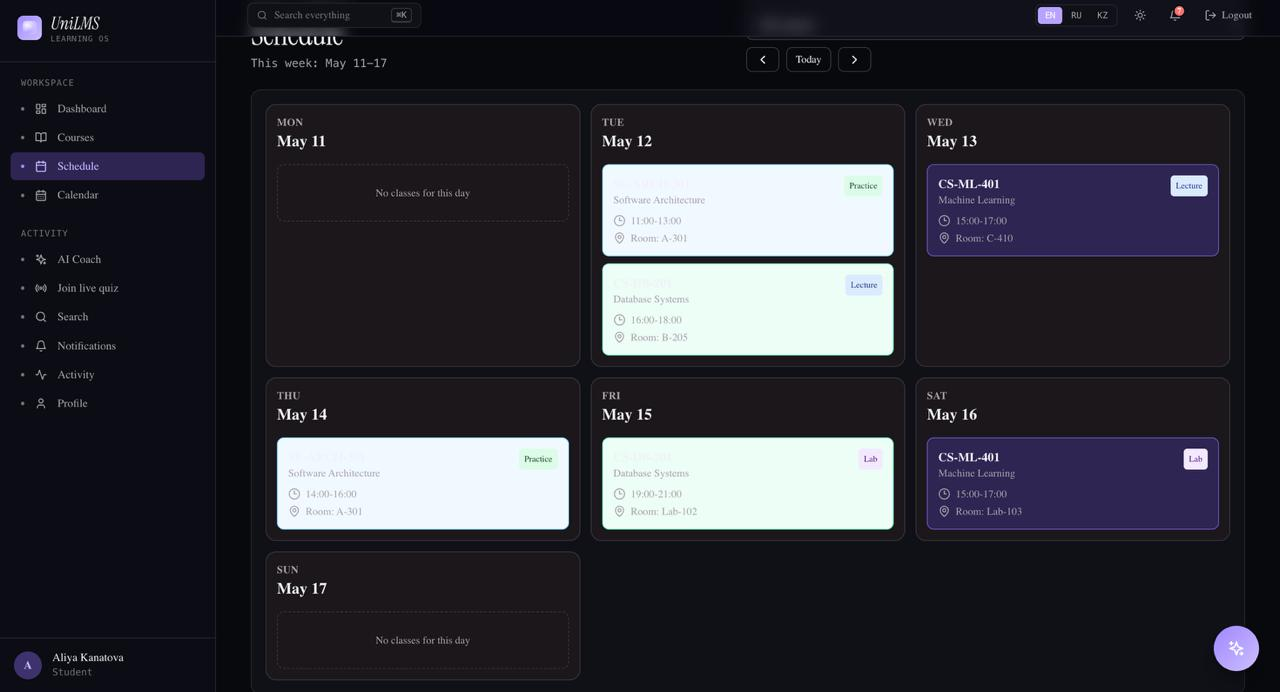
\includegraphics[width=0.85\linewidth,height=4.4cm,keepaspectratio]{figures/17-schedule.jpg}
    \caption{Weekly schedule and calendar with class, deadline, and event overlays}
\end{figure}

The schedule module unifies recurring class slots, one-off events,
assignment deadlines, and quiz windows on a single weekly grid. Dates and
times are formatted through the Intl API with the user's preferred locale,
including correct Kazakh weekday names and date abbreviations.

\begin{figure}[H]
    \centering
    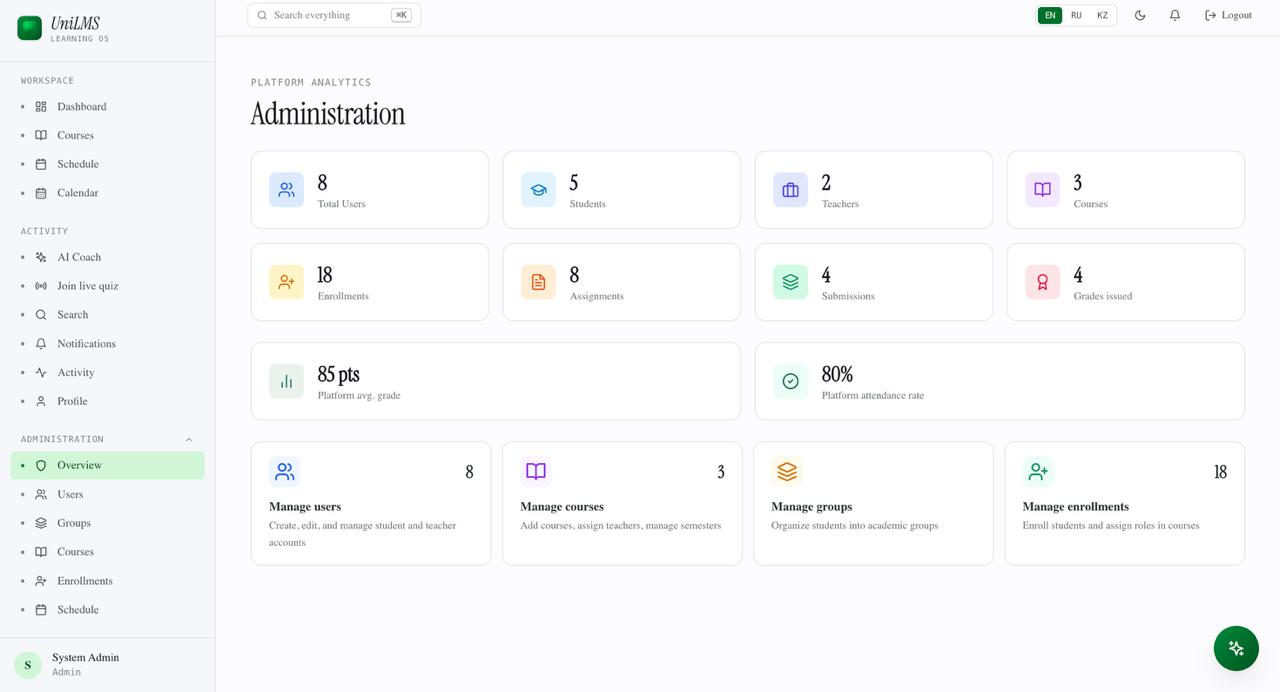
\includegraphics[width=0.85\linewidth,height=4.4cm,keepaspectratio]{figures/21-admin-dashboard.jpg}
    \caption{Administrative dashboard with platform-wide statistics}
\end{figure}

The administrative dashboard aggregates platform-wide statistics --- total
users by role, active courses, recent registrations, and AI-endpoint usage.
Every administrative action is recorded in an immutable audit log, which is
critical for accountability in a real university deployment.

\end{document}
